\setboolean{IsHalfPage}{false}%
\setboolean{IsHalfPageLeftCol}{false}%
\setboolean{IsHalfPageRightCol}{false}%
\def\ChapterTitle{%
	Kalideres Integrated Bus Terminal
}
\def\ChapterUrl{%
	https://arnottferels.github.io/work/kalideres-integrated-bus-terminal
}
\def\ChapterDescription{%
	Transforming Jakarta's Transportation Hub Towards Sustainability
}
\def\ChapterDetailsLine{%
	Bachelor's Thesis -- 2020 | Transit Design; Environmental Design; Parametric Design | West Jakarta, Indonesia
}
\def\ChapterDetailsTabular{%
	\begin{tabular}{@{}ll}
		\textbf{Type}       & Individual work                                                                         \\
		\textbf{Software}   & Rhino, Grasshopper, Ladybug Tools, Paneling Tools, Twinmotion, Photoshop \& Illustrator \\
		\textbf{Instructor} & Yaseri D. Apritasari                                                                    \\
		\textbf{URL}        & \textcolor{blue}{\footnotesize\texttt{\href{\ChapterUrl}{\ChapterUrl}}}                 \\
	\end{tabular}
}
\def\ChapterAbstract{%
	This project transforms the Kalideres Integrated Bus Terminal into a sustainable transit model for Jakarta, Indonesia. Tackling population density challenges, it introduces renewable energy, green spaces, and sustainable materials for enhanced environmental quality. The design prioritizes efficient pedestrian and vehicular movement, incorporating an overpass road and promoting universal design principles. With a strong emphasis on green transportation, the project strategically integrates eco-friendly elements, contributing to Jakarta's resilient urban infrastructure and fostering a sustainable, accessible transportation hub.
}
\StartTwoColumnLayout
\chapter*{\ChapterTitle}\addcontentsline{toc}{chapter}{\ChapterTitle}
\ChapterSetTocAddData{\ChapterDetailsLine}
\ChapterSetDetailsData{\ChapterDescription}{\ChapterDetailsLine}{\ChapterDetailsTabular}
\RuleAbstract
\ChapterAbstract
\section*{
  Issues \& Strategies
 }
%
\begin{figure}[H]
	\centering
	\includesvg[width=\linewidth]{src/graphics/kalideres-integrated-bus-terminal--issues-strat.svg}
	\label{
		fig:kalideres-integrated-bus-terminal--issues-strat
	}
\end{figure}

\vfill
\section*{
  Design Generation
 }
%
\begin{figure}[H]
	\centering
	\includesvg[width=\linewidth]{src/graphics/kalideres-integrated-bus-terminal--design-generation.svg}
	\label{
		fig:kalideres-integrated-bus-terminal--design-generation
	}
\end{figure}

\vfill
\section*{
  Environmental Analysis
 }
\setlength{\columnsep}{0.5cm}
\begin{multicols}{3}
	%
\begin{figure}[H]
	\centering
	\includesvg[width=\linewidth]{src/graphics/kalideres-integrated-bus-terminal--set-radiation-analysis.svg}
	\label{
		fig:kalideres-integrated-bus-terminal--set-radiation-analysis
	}
\end{figure}

	Radiation on the site is mainly on the roof and second floor, suitable for non-human activities. Human facilities align with climate analysis under a roof.
	\columnbreak%
	%
\begin{figure}[H]
	\centering
	\includesvg[width=\linewidth]{src/graphics/kalideres-integrated-bus-terminal--set-sunlight-hour-analysis.svg}
	\label{
		fig:kalideres-integrated-bus-terminal--set-sunlight-hour-analysis
	}
\end{figure}

	Due to its equatorial location, the site experiences substantial UV sunlight exposure (above 570~hours). However, the mezzanine floor at Level~1 receives limited UV sunlight (57 hours), suitable for introducing transitional zone functions.
	\columnbreak%
	%
\begin{figure}[H]
	\centering
	\includesvg[width=\linewidth]{src/graphics/kalideres-integrated-bus-terminal--set-spherical-view-analysis.svg}
	\label{
		fig:kalideres-integrated-bus-terminal--set-spherical-view-analysis
	}
\end{figure}

	In most areas of the site, a~75\% spherical view is achievable, except beneath the flyover, where it drops to below~35\%. The design should incorporate a dedicated express lane while maintaining a concept of continuity.
\end{multicols}
\columnbreak%
\section*{
  Design Strategy -- How Bus \& Human Circulation Works
 }
\setlength{\MinipageGap}{0.5cm}
\setlength{\MinipageAWidth}{\dimexpr0.725\linewidth -\MinipageGap}
\setlength{\MinipageBWidth}{\dimexpr\linewidth -\MinipageAWidth -\MinipageGap\relax}
\begin{minipage}[t]{\linewidth}%
	\def\FigureKalideresIntegratedBusTerminalDesignStrat{%
		\begin{minipage}[t]{\MinipageAWidth}%
			%
\begin{figure}[H]
	\centering
	\includesvg[width=\linewidth]{src/graphics/kalideres-integrated-bus-terminal--design-strat.svg}
	\label{
		fig:kalideres-integrated-bus-terminal--design-strat
	}
\end{figure}	%
%
		\end{minipage}%
	}
	\def\Figure{\FigureKalideresIntegratedBusTerminalDesignStrat}
	\settototalheight{\ContentHeight}{\Figure}
	\FigureKalideresIntegratedBusTerminalDesignStrat
	\hspace*{\MinipageGap}%
	\begin{minipage}[t][\ContentHeight][t]{\MinipageBWidth}
		\vfill
		\textbf{Flow}
		\vspace*{0.25cm}%
		\newline%
		\definecolor{orange}{HTML}{FF6900}
		\definecolor{pink}{HTML}{E4007E}
		\definecolor{red}{HTML}{FF0000}
		\definecolor{green}{HTML}{4C8700}
		\definecolor{blue}{HTML}{005AAB}
		\definecolor{lightgray}{HTML}{DADADA}
		\begin{tikzpicture}[line width=1pt, >={Latex[length=3mm]}, font=\small]
			\fill[lightgray, rounded corners=0.2cm] (-0.125,-0.25) rectangle (1.125,0.25);
			\draw[dashed, ->, draw=white, line width=1pt] (0,0) -- (1,0) node[pos=1.0, right=0.25cm] {Main Circulation (Loop)};
			\draw[dashed, <->, draw=orange] (0,-0.5) -- (1,-0.5) node[pos=1.0, right=0.25cm] {Humans \& Cyclists};
			\draw[dashed, ->, draw=pink] (0,-1) -- (1,-1) node[pos=1.0, right=0.25cm] {Parking};
			\draw[dashed, ->, draw=red] (0,-1.5) -- (1,-1.5) node[pos=1.0, right=0.25cm] {Long-distance bus};
			\draw[dashed, ->, draw=green] (0,-2) -- (1,-2) node[pos=1.0, right=0.25cm] {Local bus};
			\draw[dashed, ->, draw=blue] (0,-2.5) -- (1,-2.5) node[pos=1.0, right=0.25cm] {TransJakarta (BRT)};
		\end{tikzpicture}
		\vspace*{0.25cm}%
		\newline%
		\textbf{Function}
		\vspace*{0.25cm}%
		\newline%
		\begin{enumerate}[label=\Alph*, itemsep=0.2em, leftmargin=1.2cm]%
			\item \hspace{0.3cm}Long-distance bus
			\item \hspace{0.3cm}Local bus
			\item \hspace{0.3cm}TransJakarta (BRT)
		\end{enumerate}
		\vspace{0.25cm}
		This site plan shows the layout divided into three sections from north to south: parking for long-distance buses, a building for long-distance buses, a building for local buses, a TransJakarta bus stop, and a bridge connecting to the main road (Daan Mogot Rd). Purposeful empty spaces (void) between each bus service area ensure ample light and air circulation, preventing overcrowding.
	\end{minipage}
\end{minipage}
\vfill
\begin{minipage}[t]{\linewidth}%
	\def\FigureKalideresIntegratedBusTerminalAerial{%
		\begin{minipage}[t]{\MinipageAWidth}
			%
\begin{figure}[H]
	\centering
	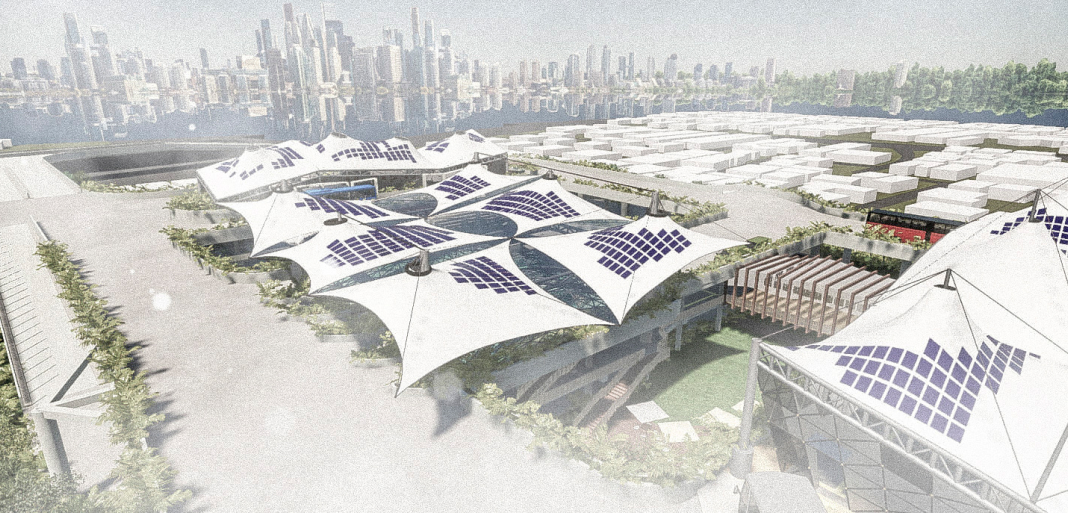
\includegraphics[width=\linewidth]{src/graphics/kalideres-integrated-bus-terminal--perspective-aerial.jpg}
	\caption*{%
		Aerial View -- Kalideres Integrated Bus Terminal
	}
	\label{
		fig:kalideres-integrated-bus-terminal--perspective-aerial
	}
\end{figure}

		\end{minipage}
	}
	\def\Figure{\FigureKalideresIntegratedBusTerminalAerial}
	\settototalheight{\ContentHeight}{\Figure}
	\FigureKalideresIntegratedBusTerminalAerial
	\hspace*{\MinipageGap}%
	\begin{minipage}[t][\ContentHeight][t]{\MinipageBWidth}
		\vfill
		Placement of lightweight solar panels on the roof of the PVTE Fabric Tensile Membrane.
		\vspace{16pt}%
		\vspace{3pt}%
	\end{minipage}
\end{minipage}
\EndTwoColumnLayoutEndMulticolsTwo %
\newpage
\noindent
\begin{specialblock}
	\section*{
	  Programs
	 }
	\setlength{\columnsep}{0.5cm}%
	\begin{multicols*}{3}
		%
\begin{figure}[H]
	\centering
	\includesvg[width=\linewidth]{src/graphics/kalideres-integrated-bus-terminal--level-01.svg}
	\caption*{%
		Level~1
	}
	\label{
		fig:kalideres-integrated-bus-terminal--level-01
	}
\end{figure}

		\vspace{0.25cm}
		On Level~1, there is a dedicated entrance for motorcycles, bicycles, and pedestrians. The parking space accommodates cars, public transportation vehicles, motorcycles, bicycles (including for firefighting and ambulances). A central area features a main lobby/midsection for drop-off and arrival areas, surrounded by a green open space called the “oasis” serving as a green area and outdoor F\&B space. The surrounding site functions as a green zone with diverse local plants.
		\vfill
		%
\begin{figure}[H]
	\centering
	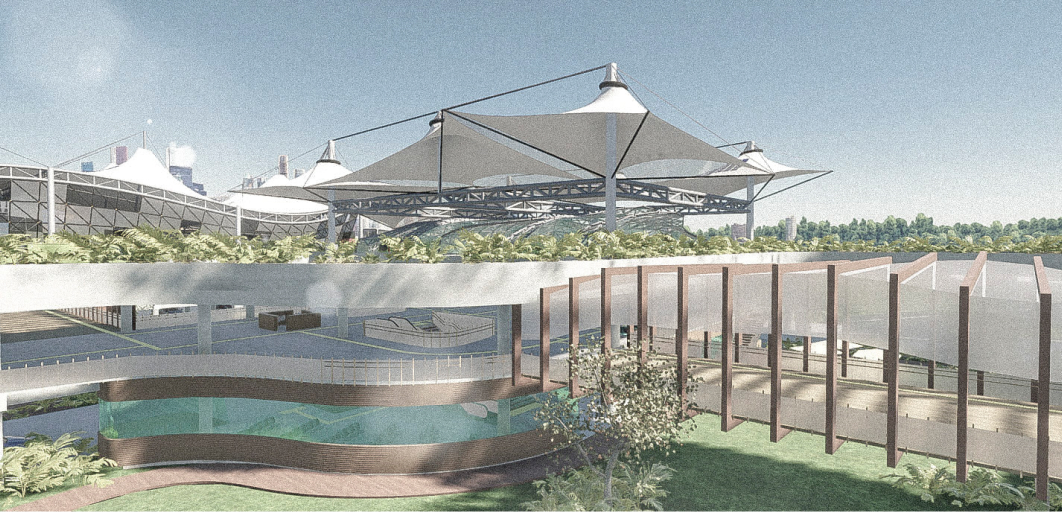
\includegraphics[width=\linewidth]{src/graphics/kalideres-integrated-bus-terminal--perspective-local-bus-bridge.jpg}
	\caption*{%
		Long-distance Bus Building \& Local Bus Terminal
	}
	\label{
		fig:kalideres-integrated-bus-terminal--perspective-local-bus-bridge
	}
\end{figure}

		\columnbreak%
		%
\begin{figure}[H]
	\centering
	\includesvg[width=\linewidth]{src/graphics/kalideres-integrated-bus-terminal--level-01m.svg}
	\caption*{%
		Level~1M
	}
	\label{
		fig:kalideres-integrated-bus-terminal--level-01m
	}
\end{figure}

		\vspace{0.25cm}
		On Level~1M, there is a main transition zone that connects the parking area and the main entrance to terminal facilities, including Inter City Bus (with ticket counters), Local Bus (with a dedicated Local Bus Lobby), TransJakarta (with a TransJakarta Lobby), F\&B Area (Commercial Retail), and Services on the North side (Management Office and Crew Room).
		\vfill
		%
\begin{figure}[H]
	\centering
	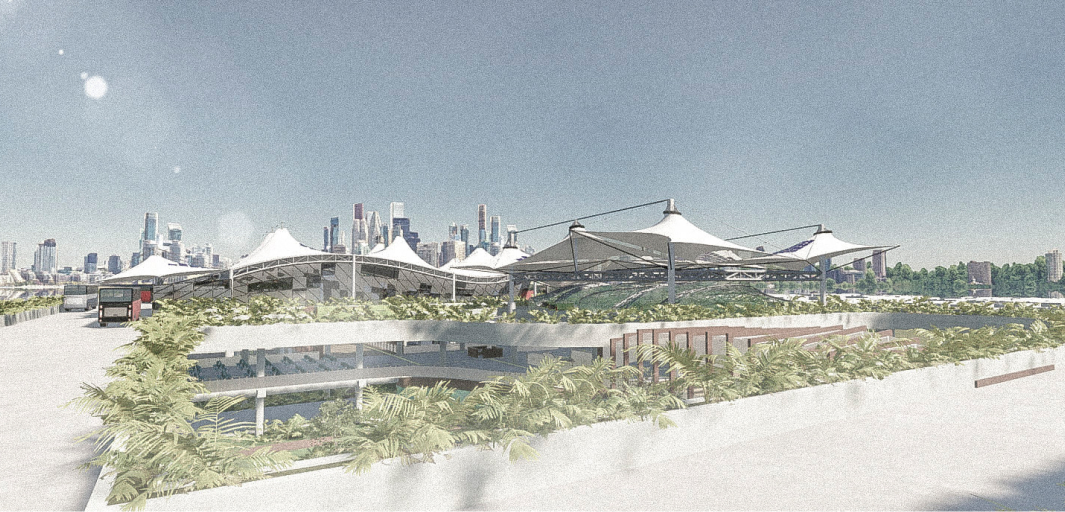
\includegraphics[width=\linewidth]{src/graphics/kalideres-integrated-bus-terminal--perspective-local-bus.jpg}
	\caption*{%
		The layers of the building that showcase various activities and zones.
	}
	\label{
		fig:kalideres-integrated-bus-terminal--perspective-local-bus
	}
\end{figure}

		\columnbreak%
		%
\begin{figure}[H]
	\centering
	\includesvg[width=\linewidth]{src/graphics/kalideres-integrated-bus-terminal--level-02.svg}
	\caption*{%
		Level~2
	}
	\label{
		fig:kalideres-integrated-bus-terminal--level-02
	}
\end{figure}

		\vspace{0.25cm}
		On Level~2, there is a dedicated circulation for vehicles accessed directly via the flyover on the South side of the terminal to avoid crossing with pedestrians. Arranged from North to South, there is a Bus Parking area, followed by the Long-distance Bus Building, Local Bus Terminal, and TransJakarta Bus Stop. There is a specific ramp directly to the first floor for parking and drop-off in the non-bus zone.
		\vfill
		%
\begin{figure}[H]
	\centering
	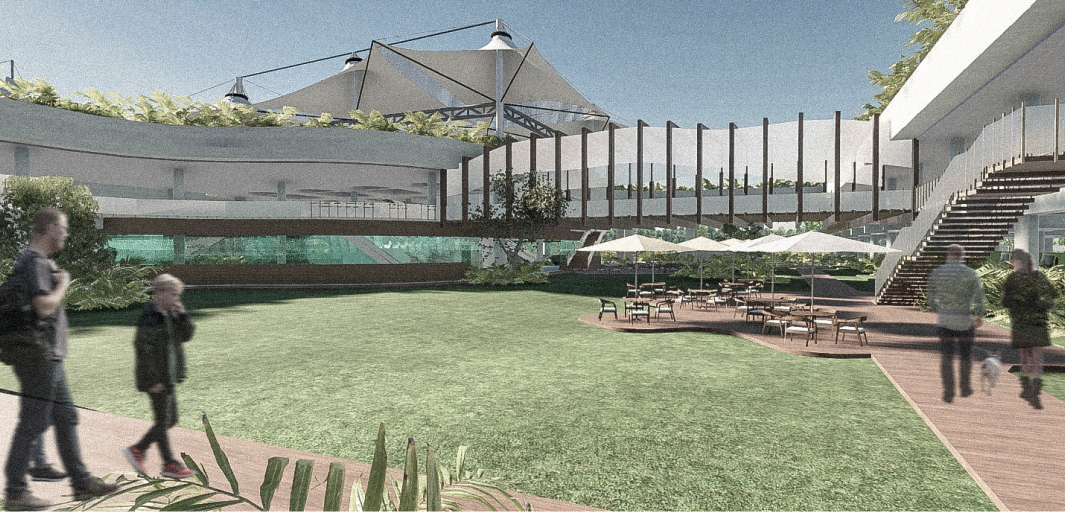
\includegraphics[width=\linewidth]{src/graphics/kalideres-integrated-bus-terminal--perspective-oasis-void-pocket.jpg}
	\caption*{%
		Open Space -- Oasis Pocket
	}
	\label{
		fig:kalideres-integrated-bus-terminal--perspective-oasis-void-pocket
	}
\end{figure}

	\end{multicols*}
\end{specialblock}
\newpage
\StartTwoColumnLayoutBeginMulticolsTwo%
\section*{
  Structural Systems \& Building Materials
 }
%
\begin{figure}[H]
	\centering
	\includesvg[width=\linewidth]{src/graphics/kalideres-integrated-bus-terminal--structural.svg}
	\label{
		fig:kalideres-integrated-bus-terminal--structural
	}
\end{figure}

The ground and mezzanine floors' parking areas and general functions are efficiently supported by a reinforced concrete structure, optimizing the parking grid module. In contrast, the platform functions for long-distance buses, local buses, and TransJakarta utilize a steel 2D truss structure with a PVTE fabric tensile membrane. The terminal design prioritizes passengers' thermal comfort, evident in the ‘oasis pocket,' an open space at the center contributing to a pleasant atmosphere.
\columnbreak%
\section*{
  Vertical Connectivity
 }
%
\begin{figure}[H]
	\centering
	\includesvg[width=\linewidth]{src/graphics/kalideres-integrated-bus-terminal--section-aa.svg}
	\caption*{%
		\raggedright
		\small
		\setstretch{1.25}%
		\textcolor{black}{%
			\textnormal{%
				Section A-A
			}
		}
	}
	\label{
		fig:kalideres-integrated-bus-terminal--section-aa
	}
\end{figure}

\vfill%
%
\begin{figure}[H]
	\centering
	\includesvg[width=\linewidth]{src/graphics/kalideres-integrated-bus-terminal--section-bb.svg}
	\caption*{%
		\raggedright
		\small
		\setstretch{1.25}%
		\textcolor{black}{%
			\textnormal{%
				Section B-B
			}
		}
	}
	\label{
		fig:kalideres-integrated-bus-terminal--section-bb
	}
\end{figure}

\vfill%
%
\begin{figure}[H]
	\centering
	\includesvg[width=\linewidth]{src/graphics/kalideres-integrated-bus-terminal--section-cc.svg}
	\caption*{%
		\raggedright
		\small
		\setstretch{1.25}%
		\textcolor{black}{%
			\textnormal{%
				Section C-C
			}
		}
	}
	\label{
		fig:kalideres-integrated-bus-terminal--section-cc
	}
\end{figure}

\EndTwoColumnLayout
\vfill%
%
\begin{figure}[H]
	\centering
	\includesvg[width=\linewidth]{src/graphics/kalideres-integrated-bus-terminal--elevation.svg}
	\caption*{%
		East Elevation
	}
	\label{
		fig:kalideres-integrated-bus-terminal--elevation
	}
\end{figure}

\newpage
